\documentclass{homework}

\name{Zhang Chi} % Replace (Student Name) with your name.
\id{2022010754}
\term{2024 Spring}
\course{Introduction to Theoretical Computer Science}
\hwnum{7}

%\hwname{(Name)}          % Uncomment and replace (Name) with the type of the
                          % homework (e.g, Assignment, Problem Set, etc.) if you
                          % don't want the document to be labeled as "Homework."
%\problemname{(Name)}     % Uncomment and replace (Name) with the desired label
                          % for problems created with the problem environment.
%\solutionname{(Name)}    % Uncomment and replace (Name) with the desired label
                          % for solutions created with the solution environment.

% Load any other packages you need here.

\begin{document}

\begin{problem}
  Let $\problemsty{D\text{-}SAT}$ be the problem of deciding if a CNF formula
  $\varphi$ has at least two satisfying assignment.
  Prove that $\problemsty{D\text{-}SAT}$ is $\NPC$.
\end{problem}

\begin{solution}
  By the NP-completeness of $\problemsty{SAT}$, we only need to prove that $\problemsty{SAT}\le_\P\problemsty{D\text{-}SAT}$. To decide whether any CNF $\varphi\in\problemsty{SAT}$, we can construct a new CNF $\phi = \varphi \land (y\lor \neg y) $ by introducing a new variable $y$. Apparently this construction can be done in polynomial time. Now we will prove that $\varphi\in\problemsty{SAT}\iff\phi\in\problemsty{D\text{-}SAT}$. If $\varphi$ is satisfiable by assignment $A=\{x_1,x_2,...,x_n\}$, Then $B_1 = \{x_1,...,x_n,y=0\}$ and $B_1 = \{x_1,...,x_n,y=1\}$ are both satisfying assignments of $\phi$. If $\varphi$ isn't satisfiable, which means $\varphi\equiv 0$, then there will be $\phi=\varphi\land (y\lor \neg y)\equiv 0$, since $0\land 1\equiv 0$. Therefore, $\varphi\in\problemsty{SAT}\iff\phi\in\problemsty{D\text{-}SAT}$, which means $\problemsty{SAT}\le_\P\problemsty{D\text{-}SAT}$ and $\problemsty{D\text{-}SAT}$ is $\NPC$. 
\end{solution}

\begin{problem}
  A coloring of a graph is an assignment of colors to vertices in a graph so
  that no adjacent vertices have the same color.
  Let $\THREECOL$ be the problem of deciding if a given graph $G$ has a coloring
  using three colors.
  \begin{parts}
    \part\label{a}
    We will consider two graph gadgets.
    First, the triangle graph enforces that the vertices have different colors
    and you can use two of the colors $\mathrm{T}$ and $\mathrm{F}$ to encode
    true and false.
    Second, the OR gadget given in the following graph implements the logical OR
    operation.
    Prove that the OR gadget has the property that (1) if both vertices $x$ and
    $y$ have color $\mathrm{F}$, then so is the vertex labeled by $x \lor y$;
    and (2) if one of them has color $\mathrm{T}$, then it is possible to assign
    $\mathrm{T}$ to the vertex $x \lor y$ in the gadget.

    \begin{figure}[htb!]
      \centering
      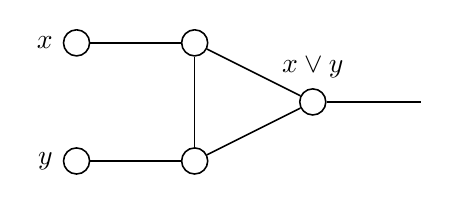
\begin{tikzpicture}[line width=.2mm]
        \pgfmathsetmacro{\h}{1.5}
        \pgfmathsetmacro{\w}{1.5}

        \node[draw,circle,label=left:{$y$}] (A0) at (0,0) {};
        \node[draw,circle,label=left:{$x$}] (B0) at (0,\h) {};

        \node[draw,circle] (A1) at (\w,0) {};
        \node[draw,circle] (B1) at (\w,\h) {};

        \node[draw,circle,label=above:{$x \lor y$}] (C) at (\w * 2,\h * .5) {};
        \node[] (D) at (\w * 3,\h * .5) {};

        \draw (A0) -- (A1);
        \draw (B0) -- (B1);
        \draw (A1) -- (B1);
        \draw (A1) -- (C);
        \draw (B1) -- (C);
        \draw (C) -- (D);
      \end{tikzpicture}
    \end{figure}

    \part\label{b}
    Use the above graph gadgets to prove that $\THREECOL$ is $\NPC$.
  \end{parts}
\end{problem}

\begin{solution}
\begin{parts}
  \part\label{2.a}
  \begin{parts}
    \part\label{2.a.1}
    Denote the five vertices of the gadget with letters shown in the graph below. 

    \begin{figure}[htb!]
      \centering
      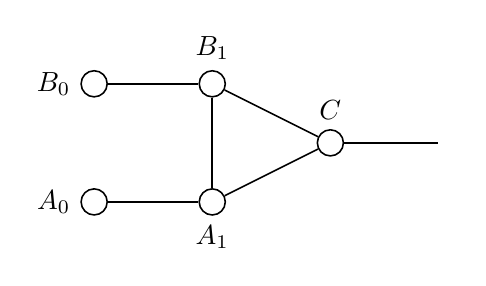
\begin{tikzpicture}[line width=.2mm]
        \pgfmathsetmacro{\h}{1.5}
        \pgfmathsetmacro{\w}{1.5}

        \node[draw,circle,label=left:{$A_0$}] (A0) at (0,0) {};
        \node[draw,circle,label=left:{$B_0$}] (B0) at (0,\h) {};

        \node[draw,circle,label=below:{$A_1$}] (A1) at (\w,0) {};
        \node[draw,circle,label=above:{$B_1$}] (B1) at (\w,\h) {};

        \node[draw,circle,label=above:{$C$}] (C) at (\w * 2,\h * .5) {};
        \node[] (D) at (\w * 3,\h * .5) {};

        \draw (A0) -- (A1);
        \draw (B0) -- (B1);
        \draw (A1) -- (B1);
        \draw (A1) -- (C);
        \draw (B1) -- (C);
        \draw (C) -- (D);
      \end{tikzpicture}
    \end{figure}
    
    Assume the three colors are $\mathrm{T}$, $\mathrm{F}$, and $\mathrm{N}$, Then if $A_0$ and $B_0$ are both colored T, $\{A_1,B_1\}=\{T,N\}$. So $C$ can't be colored with either T or N, which means it can only be colored with F.
    \part\label{2.a.2}
    Suppose $A_0$ is colored T, and $B_0$ with some unknown color $x\in\{F,N\}$. We can color $A_1$ with $x$, and $B_1$ with the third color (apart from T and $x$). Then $C$ can be colored with T.
  \end{parts}
  \part\label{2.b}
  We will prove that $\THREECOL\le_\P\problemsty{SAT}$, which means $\THREECOL$ is $\NPC$. Given a CNF formula $\varphi(x_1,x_2,...,x_n)$, we can construct a graph $G$ with the following rules:
  \begin{enumerate}
    \item Create node $N$ to symbolize color N.
    \item Create node $F$ to symbolize color F.
    \item For each variable $x_i$, create two nodes symbolizing $x_i$ and $\neg x_i$. Draw lines between $x_i$, $\neg x_i$, $N$, so $\{x_i,\neg x_i\}=\{\text{T},\text{F}\}$.
    \item For each clause $C_j = l_1\land l_2\land...\land l_k$, $l_i\in\{x_1,x_2,...,x_n,\neg x_1,...,\neg x_n\}$, use the gadget in \ref{2.a.1} to connect the relevant variables. First connect the nodes symbolizing $l_1$ and $l_2$ using the gadget, and then connect the output node $l_1\land l_2$ with $l_3$ using the gadget. Repeat this process and we can get a node symbolizing $C_j$.
    \item For the nodes symbolizing each clauses $C_j$, connect it with node $N$ and node $F$, which restricts the clause to be colored $T$.
  \end{enumerate}
  Now, we will prove that $\varphi\in\problemsty{SAT}\iff G\in\THREECOL$. 

  First, if $\varphi$ is satisfiable, then we can color the variables with T and F according to the satisfying assignment and color the clause nodes with T. In the satisfying assignment, every clause has at least one true variable, so the output node of the gadget can be colored with T since in \ref{2.a.2} we've proved that the output node can be colored with T if one of its input is T. We color node $N$ to N and node $F$ to F, and since all clause nodes are colored T there are no adjacent vertices with the same color. Therefore, $G\in\THREECOL$.

  Second, if $G\in\THREECOL$, we name the color of node $N$ as N, and the color of node $F$ as F. Since all clause nodes are connected to $N$ and $F$, so they all need to be colored in T. Meanwhile, in \ref{2.a.1} we've proved that the output node will be F if all input nodes are F, so at least one of the input nodes of each clause must be colored T. If node symbolizing $x_i$ is colored T, Then the node for $\neg x_i$ must be F since they are connected with each other and both with $N$. Therefore, we can assign "true" to all variables whose corresponding nodes are colored with T in $G$. This will ensure that $\forall i,x_i\neq\neg x_i$ and that all clauses have at least one true variable, which satisfies $\varphi$. 
  
  Therefore, $\varphi\in\problemsty{SAT}\iff G\in\THREECOL$, which indicates $\THREECOL$ is $\NPC$.
\end{parts}
\end{solution}

\begin{problem}
  Write a complete proof for the Claim 1 in the proof of Ladner's theorem
  discussed in class.
  That is, show that both $Z(n)$ and $n^{Z(n)}$ are computable in time
  polynomial in $n$.
  The definition of $Z(n)$ is given in the lecture notes.
\end{problem}

\begin{solution}
  We compute $Z(n)$ recursively. Suppose $Z(n-1)=i$, then if $M_i$ can compute $\SAT_Z(x)$ for all $x$ with $|x|<\log n$ in $|x|^i$ time, let $Z(n)=Z(n-1)$. Else, let $Z(n)=\min\{Z(n-1)+1,\log\log n\}$.
  
  There exist at most $O(2^{\log n}) = O(n)$ kinds of input with length $\log n$, so for the simulation to get $Z(n)$ from $Z(n-1)$, we need at most $O(|x|^i\times n)\le O(n(\log n)^{Z(n-1)})\le O(n(\log n)^{\log log n})$ time. By the fact that $\log x<\sqrt{x}$ if $x$ is large enough, we have, with large enough $n$, $\log\bigl((\log n)^{\log\log n}\bigr)= (\log\log n)^2<\log n$ (take $x=\log n$ in the above inequality). So, the above time complexity $O(n(\log n)^{\log log n}) = O\bigl(n\times 2^{\log((\log n)^{\log\log n})}\bigr) < O(n\times 2^{\log n}) = O(n^2)$. 
  
  Therfore, to compute $Z(n)$ from scratch, we need to compute $Z(1)$, $Z(2)$, ..., $Z(n)$ in order. So the total time complexity is at most $\sum_{k=1}^n O(k^2) = O(n^3)$, which means $Z(n)$ is polynomial-time (of $n$) constructible.

  Since $Z(n)$ can be computed in $O(n^3)$ time, we can compute $n^{Z(n)}$ by the fast-exponentiation algorithm. We only need $O(\log(Z(n)))\le O(\log\log\log n)$ amount of multiplication, each with multipliers less than $n^{Z(n)}\le n^{\log\log n}$. So the length of the multipliers are at most $l=\log(n^{\log\log n}) = \log n\log\log n$, and each multiplication can be done in $O(l^2) < O((\log n)^4)$ complexity. Therefore, the total complexity is at most $O(\log\log\log n \times (\log n)^4)< O((\log n)^5)< O(n)$, which means $n^{Z(n)}$ is also computable in polynomial time of $n$.
\end{solution}

\end{document}
